\documentclass{article}


% if you need to pass options to natbib, use, e.g.:
%     \PassOptionsToPackage{numbers, compress}{natbib}
% before loading neurips_2022


% ready for submission
\usepackage{neurips_2022}


% to compile a preprint version, e.g., for submission to arXiv, add add the
% [preprint] option:
%     \usepackage[preprint]{neurips_2022}


% to compile a camera-ready version, add the [final] option, e.g.:
%     \usepackage[final]{neurips_2022}


% to avoid loading the natbib package, add option nonatbib:
%    \usepackage[nonatbib]{neurips_2022}

\usepackage{listings}
\usepackage{pdfpages}
\usepackage{xcolor}
\usepackage{lmodern}
\usepackage{amssymb}
\usepackage{placeins}
\usepackage{float}
\usepackage{graphicx}
\usepackage{subfig}
\usepackage{indentfirst}
\usepackage{color}
\usepackage{graphicx}
\usepackage{microtype}
\usepackage{amsmath}
\usepackage{amsfonts}
\usepackage{tikz}
\usetikzlibrary{shapes, shadows, arrows}
\usepackage{acronym}
\usepackage[utf8]{inputenc} % allow utf-8 input
\usepackage[T1]{fontenc}    % use 8-bit T1 fonts
\usepackage{hyperref}       % hyperlinks
\usepackage{url}            % simple URL typesetting
\usepackage{booktabs}       % professional-quality tables
\usepackage{amsfonts}       % blackboard math symbols
\usepackage{nicefrac}       % compact symbols for 1/2, etc.
\usepackage{microtype}      % microtypography
\usepackage{xcolor}         % colors


\title{Do we need more bikes? Project in Machine Learning}


% The \author macro works with any number of authors. There are two commands
% used to separate the names and addresses of multiple authors: \And and \AND.
%
% Using \And between authors leaves it to LaTeX to determine where to break the
% lines. Using \AND forces a line break at that point. So, if LaTeX puts 3 of 4
% authors names on the first line, and the last on the second line, try using
% \AND instead of \And before the third author name.


\author{%
  David S.~Hippocampu\thanks{Use footnote for providing further information
    about author (webpage, alternative address)---\emph{not} for acknowledging
    funding agencies.} \\
  Department of Computer Science\\
  Cranberry-Lemon University\\
  Pittsburgh, PA 15213 \\
  \texttt{hippo@cs.cranberry-lemon.edu} \\
  % examples of more authors
  % Coauthor \\
  % Affiliation \\
  % Address \\
  % \texttt{email} \\
  % \AND
  % Coauthor \\
  % Affiliation \\
  % Address \\
  % \texttt{email} \\
  % \And
  % Coauthor \\
  % Affiliation \\
  % Address \\
  % \texttt{email} \\
  % \And
  % Coauthor \\
  % Affiliation \\
  % Address \\
  % \texttt{email} \\
}

\usepackage{xcolor}
\definecolor{codegreen}{rgb}{0,0.6,0}
\definecolor{codegray}{rgb}{0.5,0.5,0.5}
\definecolor{codepurple}{rgb}{0.58,0,0.82}
\definecolor{backcolour}{rgb}{0.95,0.95,0.92}
\usepackage{listings}
\lstdefinestyle{mystyle}{
backgroundcolor=\color{backcolour},
commentstyle=\color{codegreen},
keywordstyle=\color{magenta},
numberstyle=\tiny\color{codegray},
stringstyle=\color{codepurple},
basicstyle=\footnotesize\ttfamily,
breakatwhitespace=false,
breaklines=true, captionpos=b,
keepspaces=true, numbers=left,
numbersep=5pt, showspaces=false,
showstringspaces=false,
showtabs=false, tabsize=2,
}
\lstset{style=mystyle}



\begin{document}


\maketitle


\begin{abstract}
   This documents contains the analysis base on the provided data in order to solve the District Department of Transportation in Washington D.C. problem using statistical methods and reasoning to come up with an appropriate machine learning model for predicting the bike demand. The following models were implemented: Logistic Regression, Discriminant analysis (LDA and QDA), K-nearest neighbor, Tree-based methods (classification trees, random forests, bagging) and Boosting (adaptative and gradient). The goal is to find the most suitable model to predict the given problem.

\end{abstract}

\section{Introduction}

This report presents our findings of our project for the Statistical Machine Learning course, 1RT700 at Uppsala University, which intersects the domains of machine learning and urban planning.
We were presented with a sample dataset consisting of 1600 data points. The data points themselves consisted of 15 features, both categorical and numerical, as well as one categorical feature to predict.
The goal of the project was to predict if there was a need to increase supply of bikes, or not. The categorical feature we predicted for could have the value high\_demand or low\_demand, consequently making this a classification problem.
Our challenge was to dissect the data, figure out what preprocessing would make sense for the task at hand, and then use various machine learning models and methods taught in the course, to then predict the bike demand.

\section{Data analysis task}
\label{headings}

It is important to evaluate the different types of data in order to do the correct data analysis. The dataset presents three different types of data: numerical variables, categorical variables and, binary ad ordinal variables. Each of the types mentioned should be treated differently.

\begin{enumerate}
\item Which are the numerical features and which are the categorical features? 

The dataset was separated between numerical features (continuous features and discrete features) and categorical features (nominal and ordinal features).
The numerical features are the features which have an inherent ordering, based on some quantitative trait. It can be separated in continuous variables and discrete variables as can be see in Figure \ref{fig:numerical}. The numeral features can be seen bellow:

\begin{equation}
temp, dew, humidity, precip, snow, snowdepth, windspeed,
cloudcover, visibility
\label{eq:1}
\end{equation}

\begin{figure}[H]
		\centering
		\caption{Types of numerical features.}
		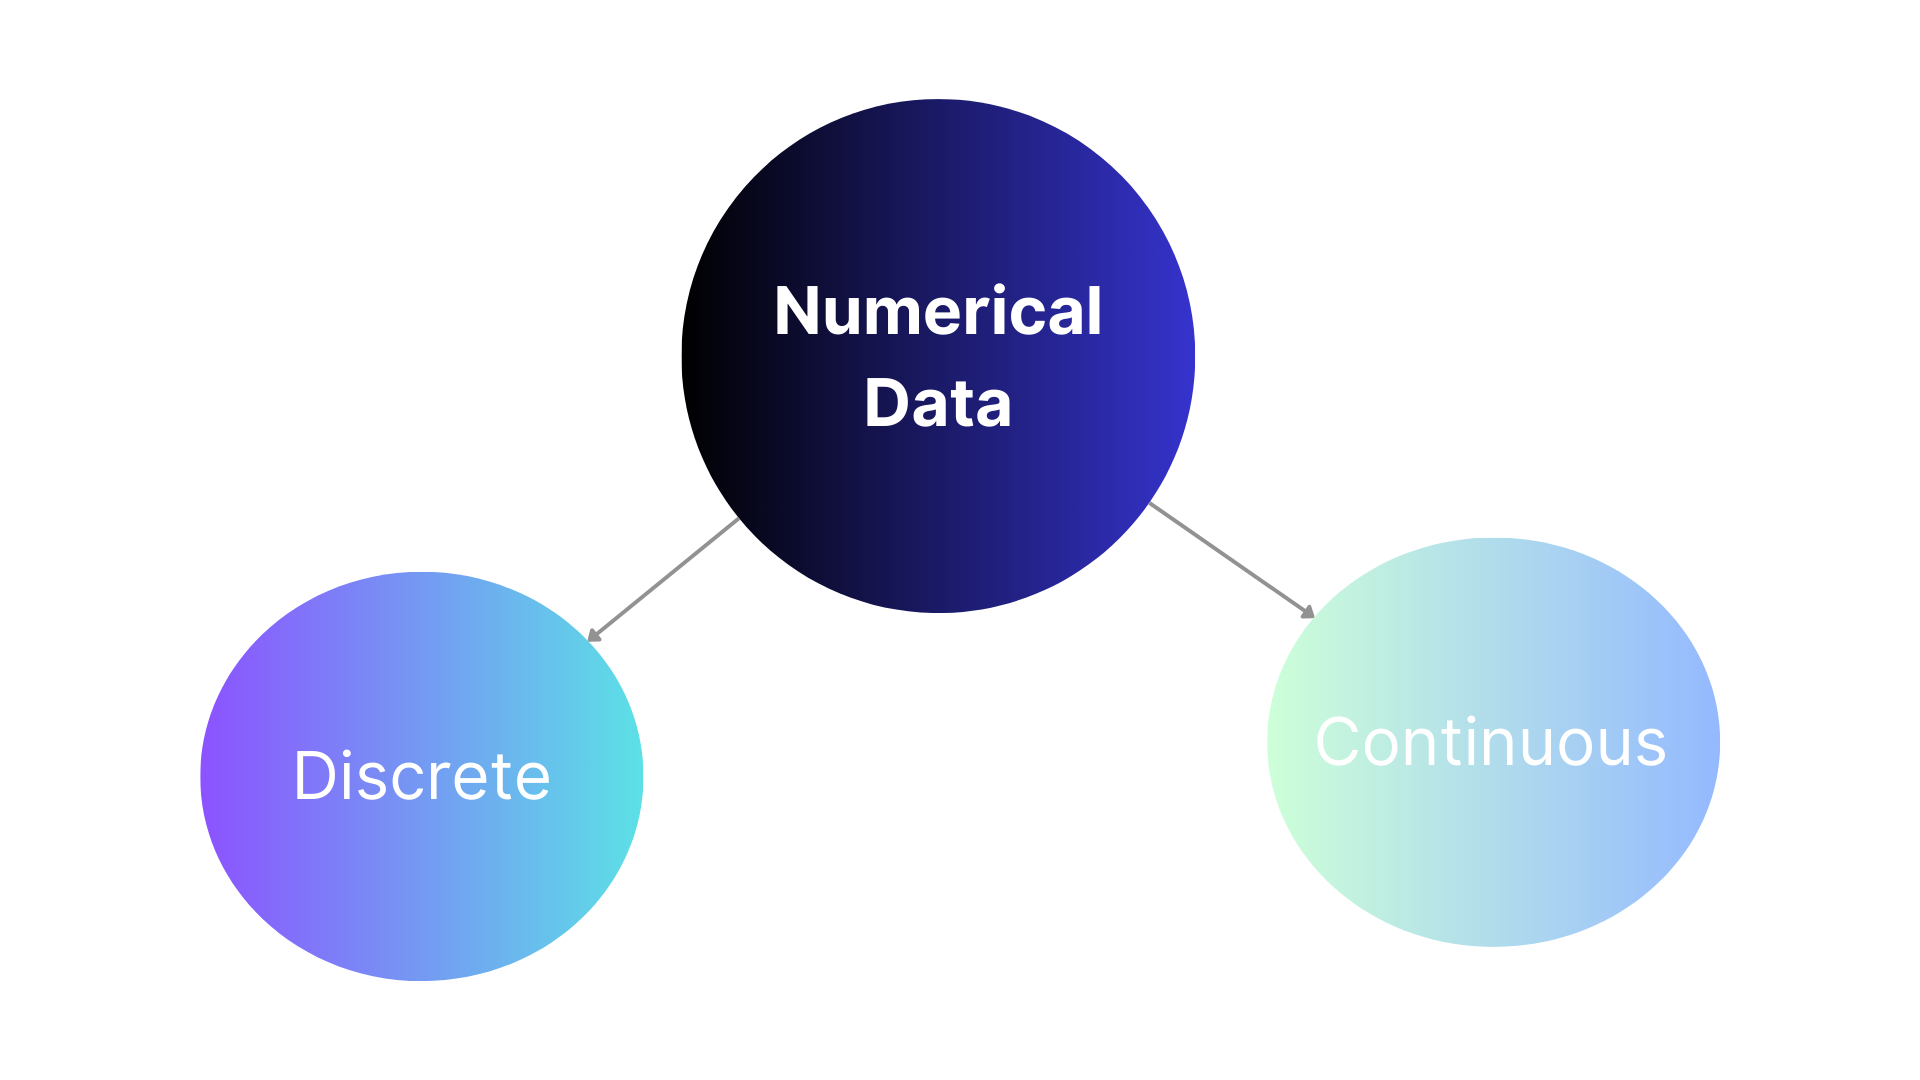
\includegraphics[width=0.5\linewidth]{Report/Images/NumericalData.png}
	\label{fig:numerical}
	\end{figure}

The continuous features are ideal for histograms because they can take on an infinite number of values within a range. The discrete features are often more appropriate for bar charts. 

%The relation between probability density and the continuous numerical features can be seen in Figure \ref{fig:1} and \ref{fig:2}.

%\begin{figure}[htb!]
%\caption{Numerical features - temp, dew, humidity.}
%\label{fig:1}
    
%\subfloat[\label{P1}temperature]{
        %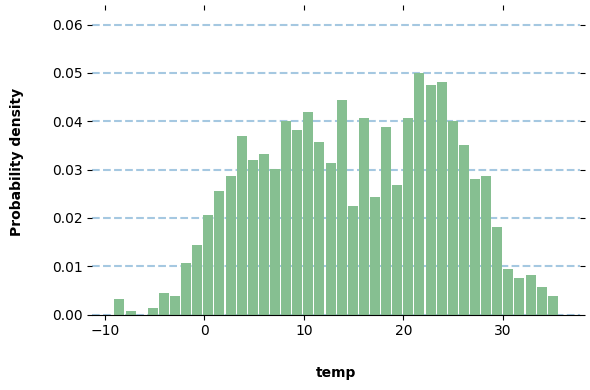
\includegraphics[width=0.3\textwidth]{Code/Plots/probability_density_temp.png}
    %}\hfill
     %\subfloat[\label{P2}dew]{
        %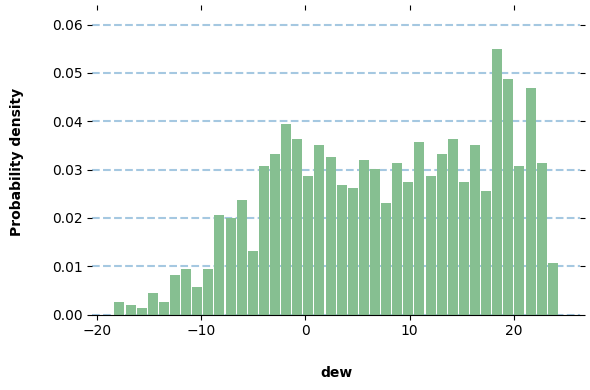
\includegraphics[width=0.3\textwidth]{Code/Plots/probability_density_dew.png}
   %} \hfill
        %\subfloat[\label{P3}humidity]{
       % 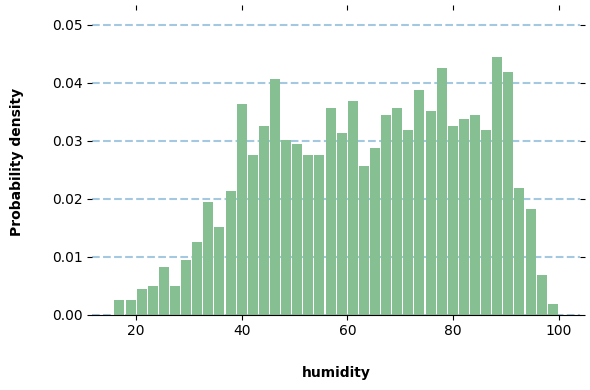
\includegraphics[width=0.3\textwidth]{Code/Plots/probability_density_humidity.png}
    % }
     
%\end{figure}

%\begin{figure}[htb!]
%\caption{Numerical features - cloudcover and windspeed.}
%\label{fig:2}
    
%\subfloat[\label{P4}cloudcover]{
       % 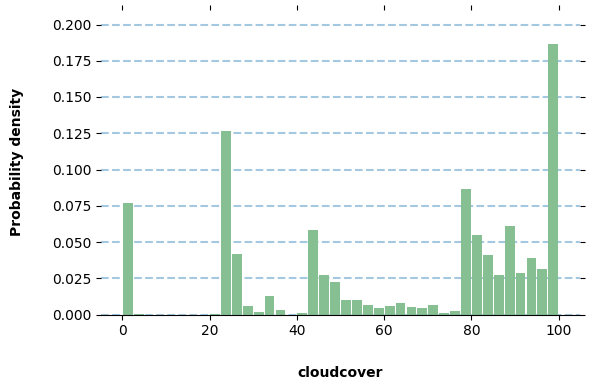
\includegraphics[width=0.4\textwidth]{Code/Plots%/probability_density_cloudcover.png}
   % }\hfill
     %\subfloat[\label{P5}windspeed]{
       % 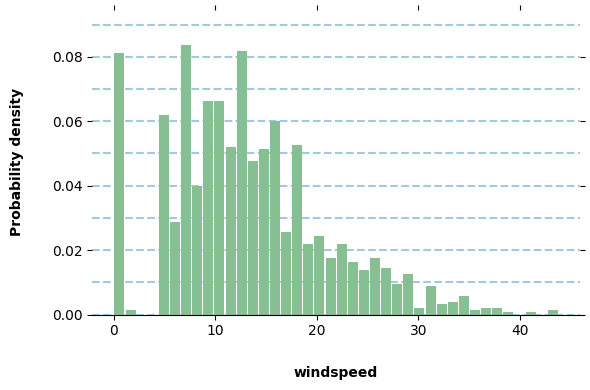
\includegraphics[width=0.4\textwidth]{Code/Plots/probability_density_windspeed.png}
    %} 
     
%\end{figure}


The correlation matrix was created for the numerical features, can be seen in the Figure \ref{fig:4}. It is possible to analyse the correlation coefficient (negative and positive) between the numerical features, it can helps to visualize pattern in the given dataset. It is possible to see the perfect correlation when the same type of feature is compared representing by the main diagonal. If the correlation between two different features is more close to the perfect correlation, means that the influence between it is high.

\begin{figure}[H]
		\centering
		\caption{Correlation matrix - numerical features.}
		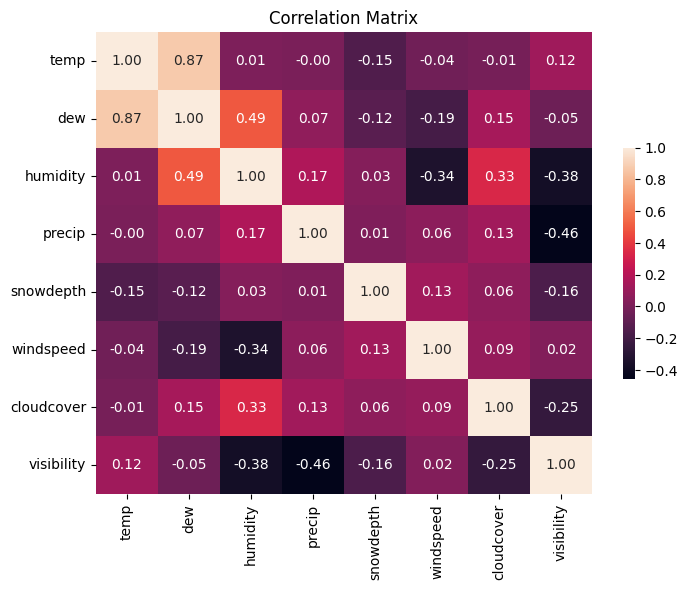
\includegraphics[width=0.7\linewidth]{Code/Plots/correlation_matriz.png}
	\label{fig:4}
	\end{figure}


   


In the categorical features there is no inherent ordering. it is based on some qualitative trait. The categorical features can be nominal or ordinal features as can be seen in Figure \ref{fig:categorical}. In this case, the given output is a categorical feature, and it can be seen bellow:

\begin{equation}
increase \textunderscore stock
\label{eq:2}
\end{equation}

\begin{figure}[H]
		\centering
		\caption{Types of categorical features.}
		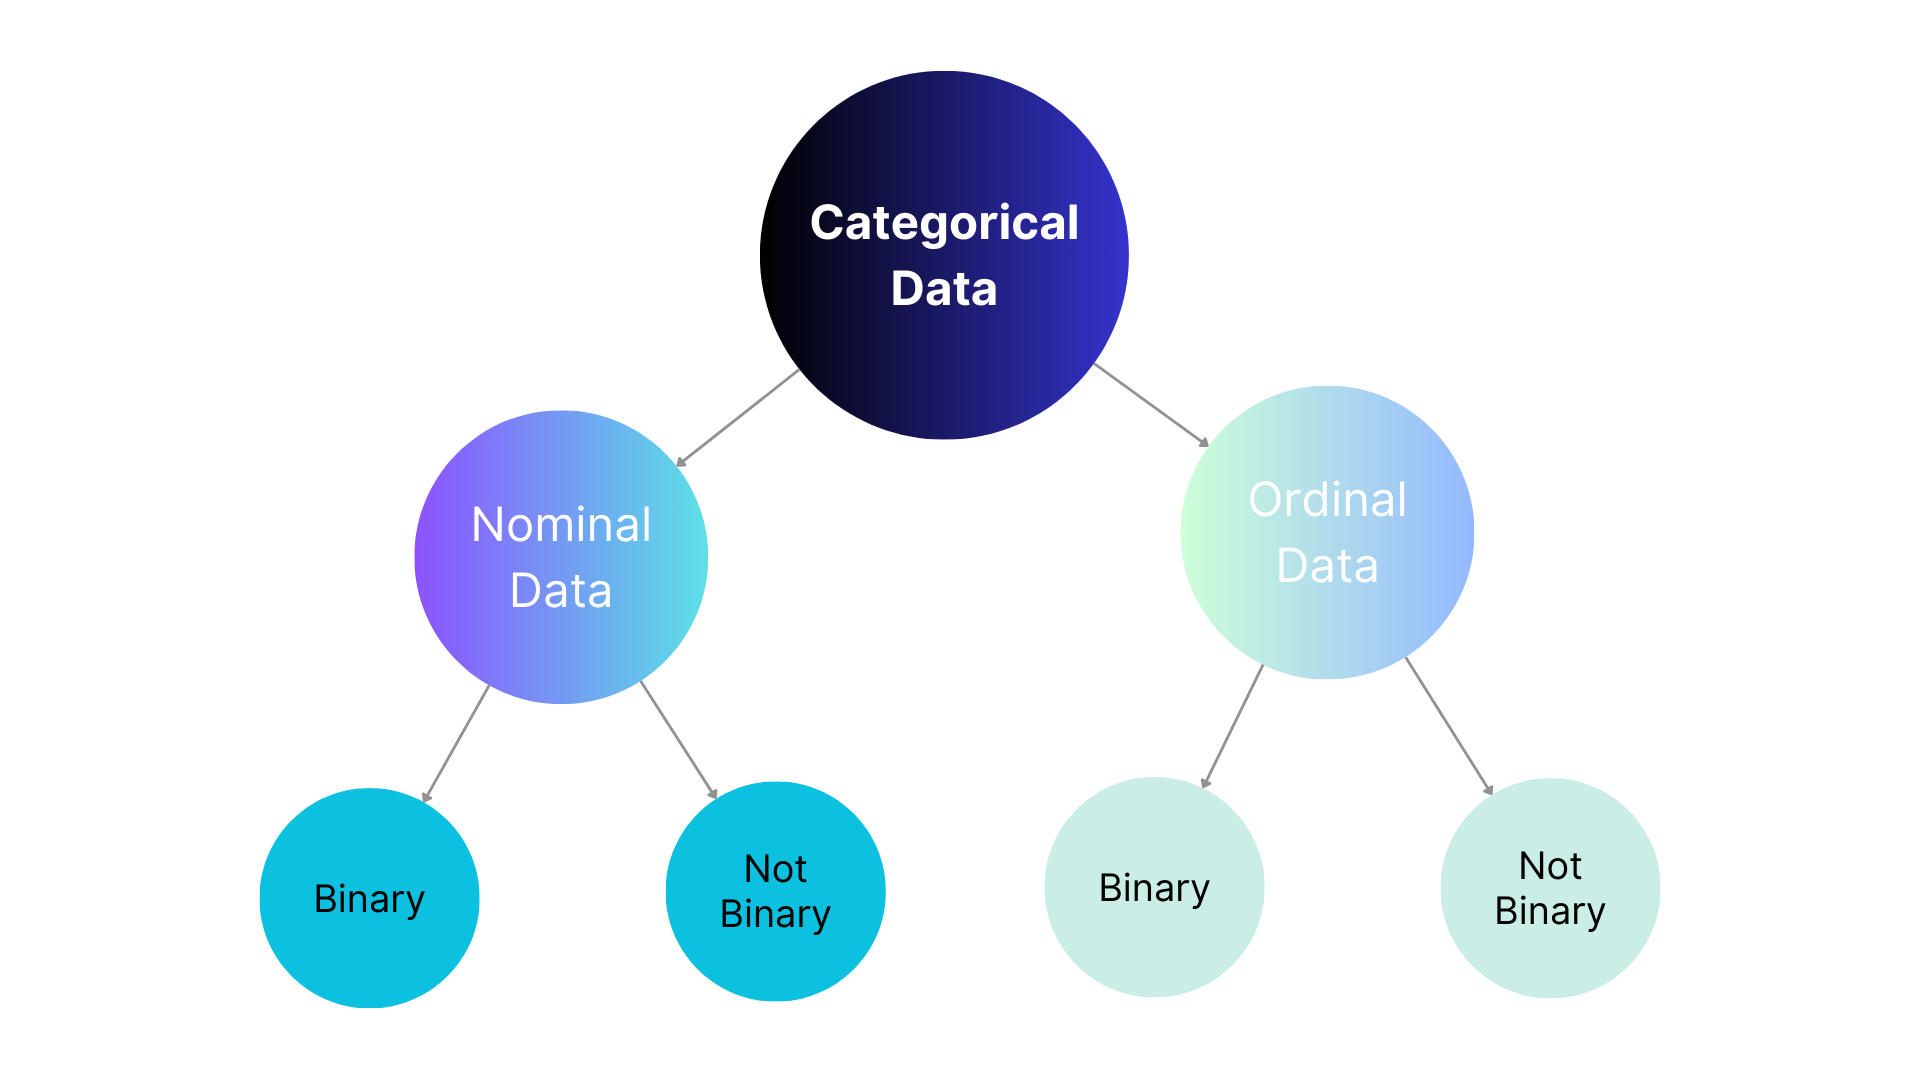
\includegraphics[width=0.7\linewidth]{Report/Images/CategoricalData.png}
	\label{fig:categorical}
	\end{figure}



 The output of the predictions is a categorical feature in the given dataset as mentioned above. The given data was analysed and it is possible to see in the code that the probability to happen the low \textunderscore bike \textunderscore demand is 82\%, and the probability to happen the high \textunderscore bike \textunderscore demand is 18\%.

 %\begin{figure}[H]
 %\centering
%\caption{The categorical feature probability.}
%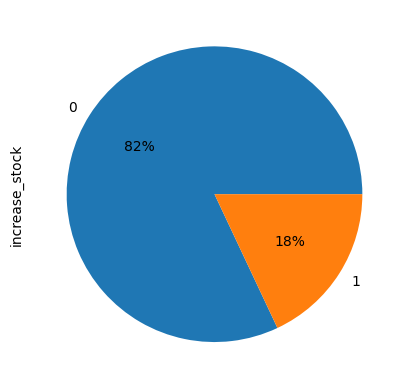
\includegraphics[width=0.5\linewidth]{Code/Plots/increase_stock.png}
%\label{fig:4}
%\end{figure}

 

The categorical features that are ordinal and binary features can be seen bellow:

\begin{equation}
hour \textunderscore of \textunderscore day, day \textunderscore of \textunderscore week, month, holiday, weekday, summertime
\label{eq:3}
\end{equation}

The binary features are only two categories, for example, Yes/No or True/False. Histograms are not usually used for binary variables because there are only two bars to display, which does not convey much information about distribution. Instead, a bar chart or pie chart might be used.

The ordinal features have a set order, for example, poor to excellent, but the intervals between the categories are not necessarily equal. Histograms can be used with ordinal data; however, the ordered nature of the data must be preserved in the bins of the histogram, and often a bar chart is clearer.

\item Is there a greater trend to need an increase in the availability of bicycles?
\begin{enumerate}
\item Can any trend be seen comparing different hours, weeks, and months?
\item Is there any difference between weekdays and holidays?
Plotting the hours of the day during weekdays against the increase stock feature shows an increase in demand for bicycles during the rush-hour windows six to nine in the morning and three to seven in the afternoon. This is illustrated in figure \ref{fig:weekday_increase_stock}.

\begin{figure}[htb!]
\caption{Days hours and weekdays.}
\label{fig:H}
\subfloat[\label{fig:weekday_increase_stock}Increase stock during day hours.]{
        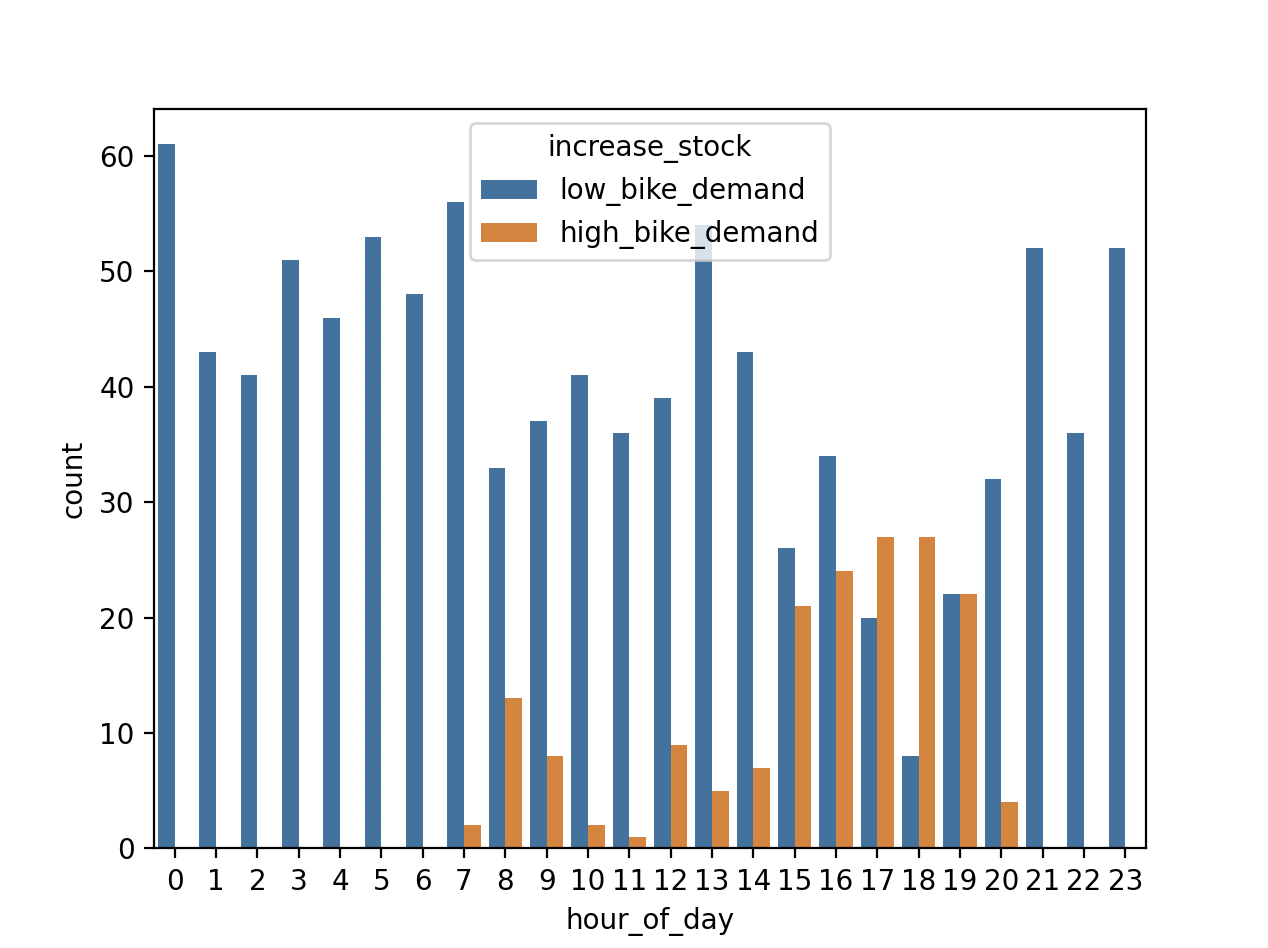
\includegraphics[width=0.5\textwidth]{Code/Plots/hour_of_day_against_increase_stock_weekday.png}
   }\hfill
     \subfloat[\label{fig:week_increase_stock}Increase stock during weekdays.]{
       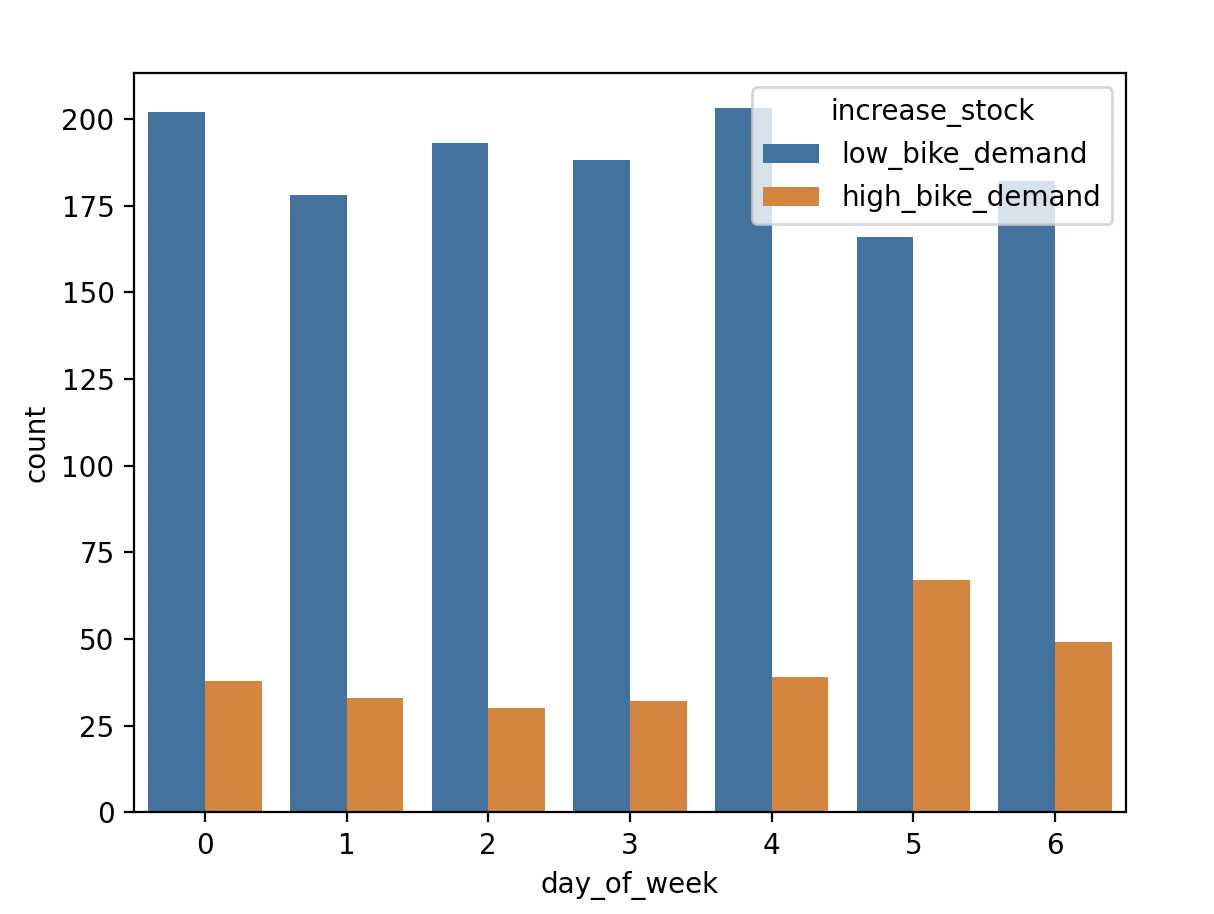
\includegraphics[width=0.5\textwidth]{Code/Plots/day_of_week_against_increase_stock.png}
    }      
\end{figure}

%\begin{figure}[htb!]
%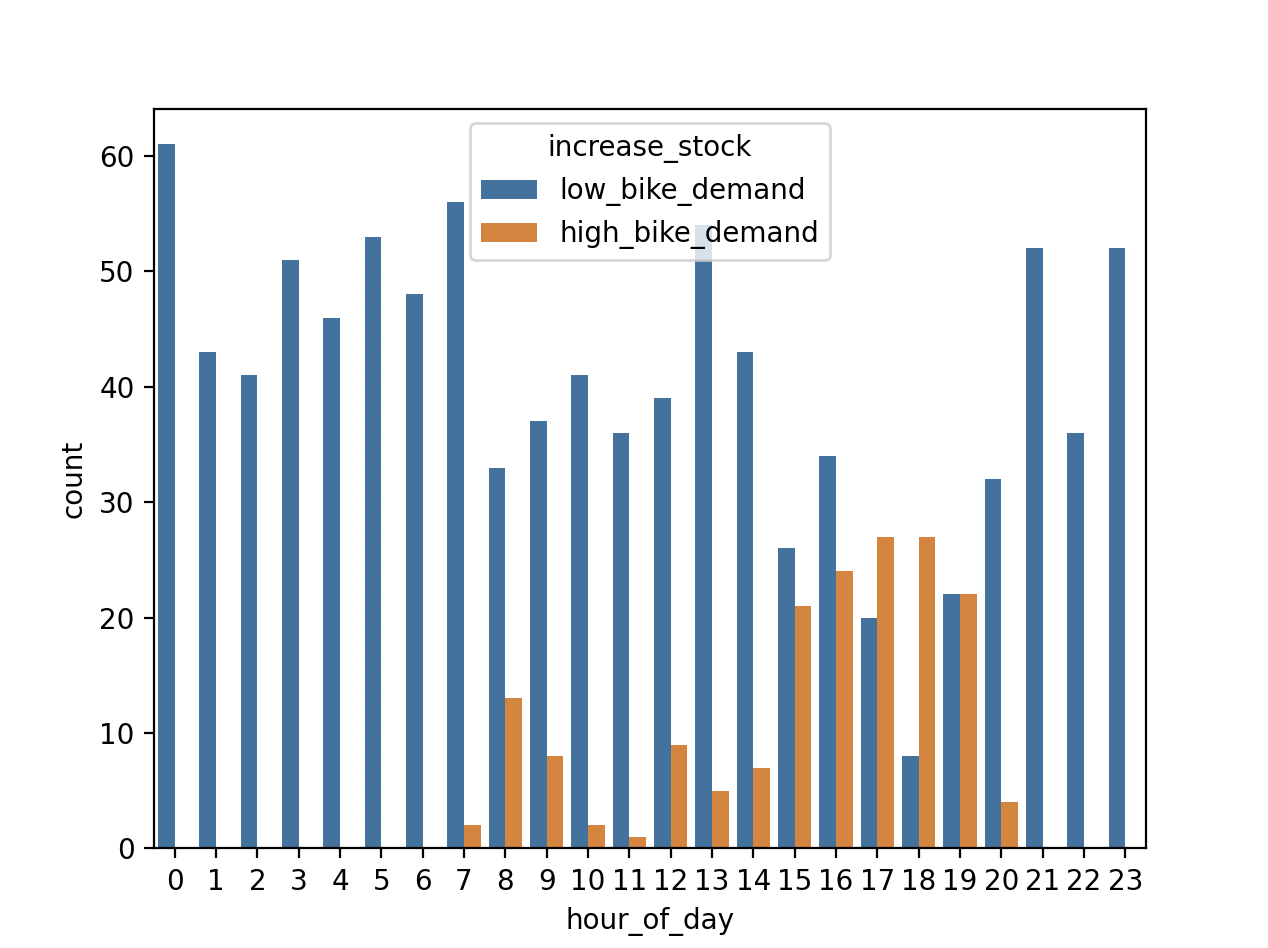
\includegraphics[width=12cm]{Code/Plots/hour_of_day_against_increase_stock_weekday.png}
%\caption{Increase stock during day hours.}
%\label{fig:weekday_increase_stock}
%\end{figure}

%\begin{figure}[htb!]
%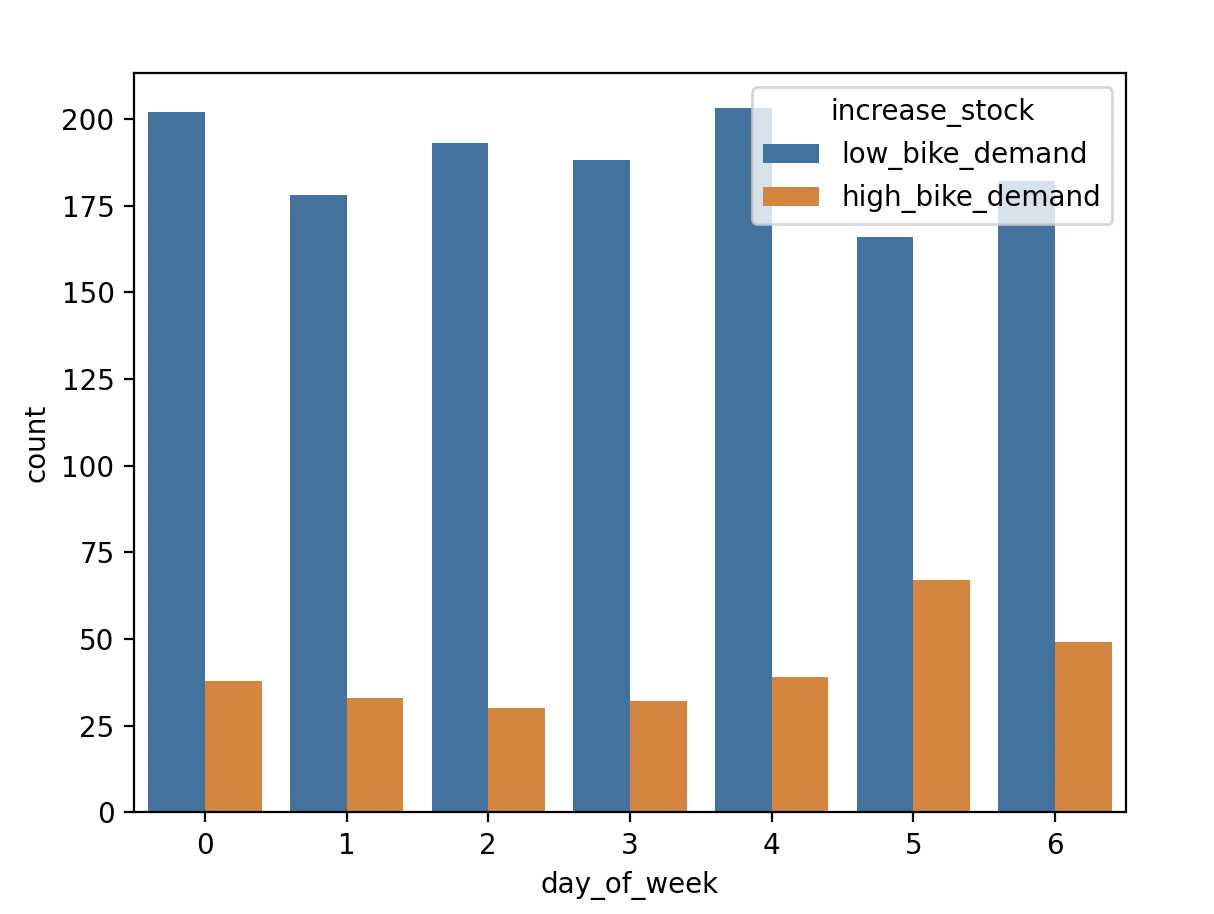
\includegraphics[width=12cm]{Code/Plots/day_of_week_against_increase_stock.png}
%\caption{Increase stock during weekdays.}
%\label{fig:week_increase_stock}
%\end{figure}

Plotting the days of the week against the increase stock feature shows an increase in demand for bicycles during the day '5' (Saturday) and '6' (Sunday) of the week. It can be seen in Figure \ref{fig:week_increase_stock}.



Plotting the months in the year against the increase stock feature shows peaks in demand for bicycles during April, June and September. It can be seen in Figure \ref{fig:months_increase_stock}.

\begin{figure}[htb!]
\caption{Months and holidays.}
\label{fig:H}
\subfloat[\label{fig:months_increase_stock}Increase stock during months.]{
        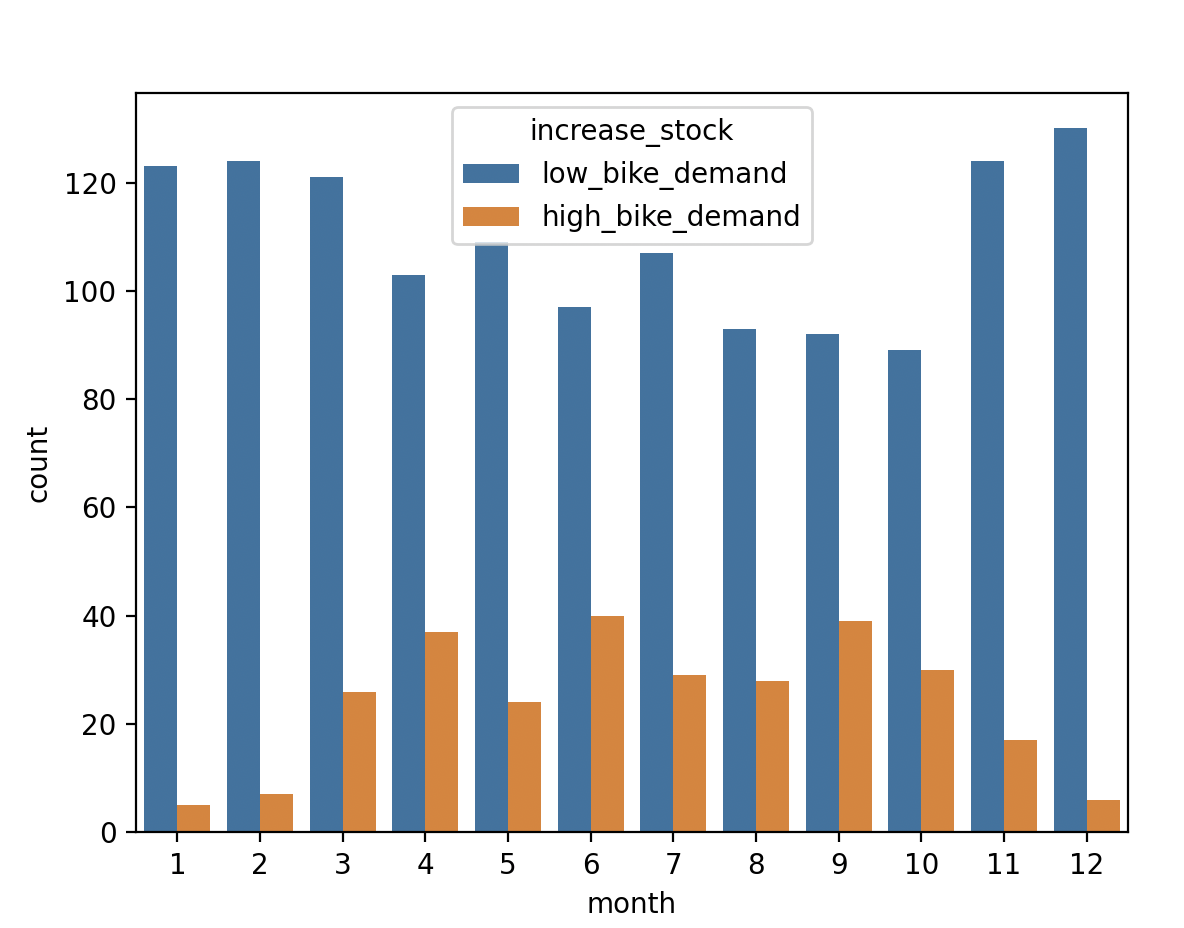
\includegraphics[width=0.5\textwidth]{Code/Plots/month_against_increase_stock.png}
   }\hfill
     \subfloat[\label{fig:holiday_increase_stock}Increase stock during holidays.]{
       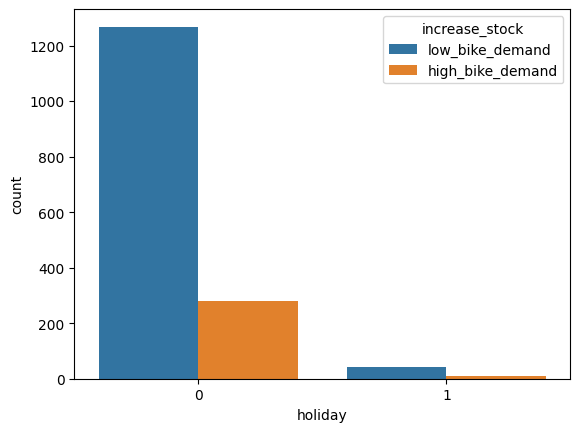
\includegraphics[width=0.5\textwidth]{Code/Plots/holiday_against_increase_stock.png}
    }      
\end{figure}

%\begin{figure}[htb!]
%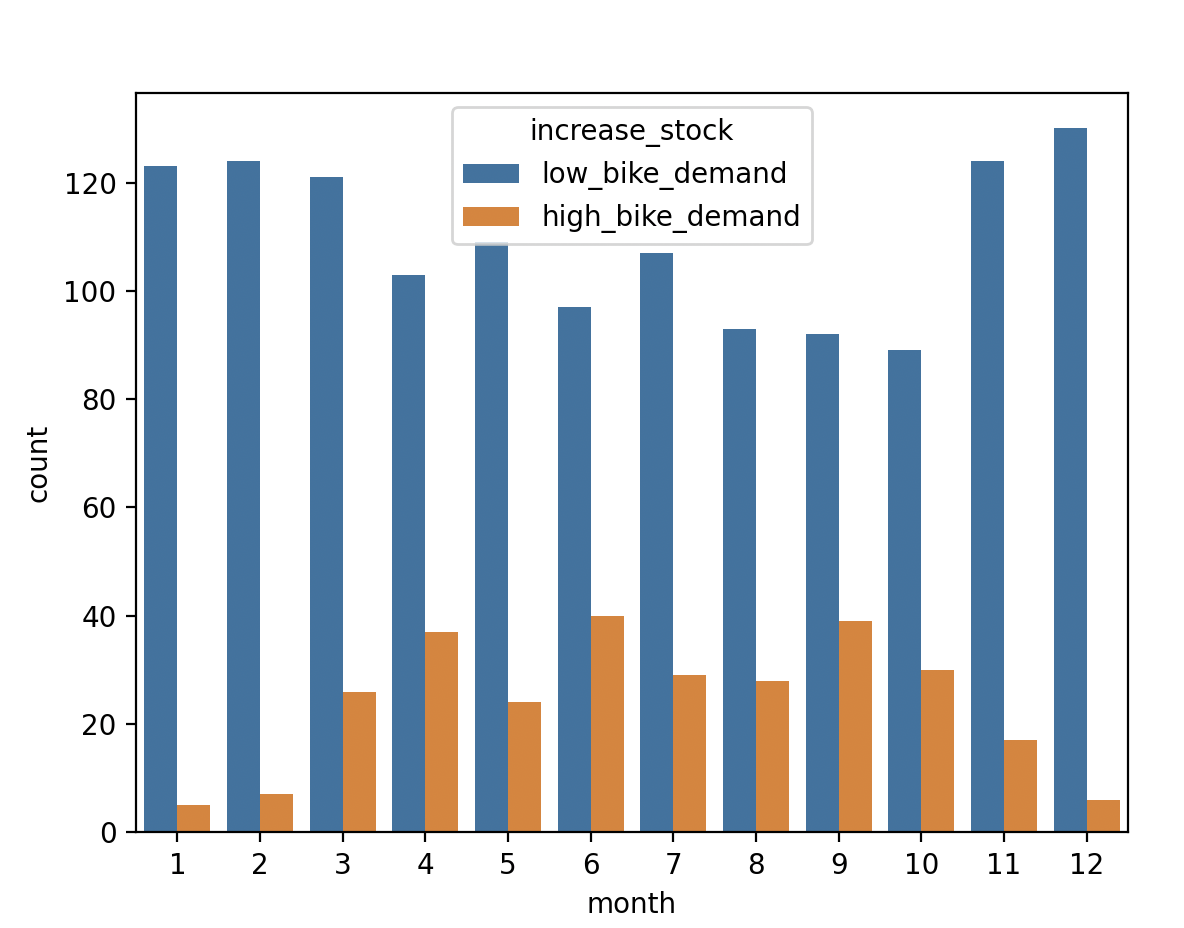
\includegraphics[width=12cm]{Code/Plots/month_against_increase_stock.png}
%\caption{Increase stock during months.}
%\label{fig:months_increase_stock}
%\end{figure}

%\begin{figure}[htb!]
%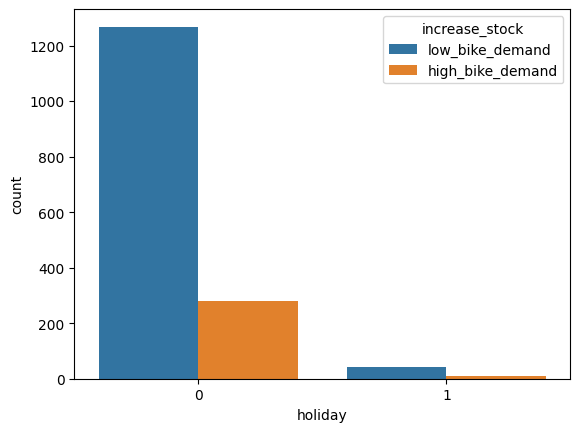
\includegraphics[width=12cm]{Code/Plots/holiday_against_increase_stock.png}
%\caption{Increase stock during holidays.}
%\label{fig:holiday_increase_stock}
%\end{figure}

It can be seen the trend when it is weekdays and holidays in Figure \ref{fig:holiday_increase_stock}. The '0' represent the weekdays and the '1' represent the holidays. The higher demand increased in weekdays compared with the holidays.


\item Is there any trend depending on the weather? Rainy days, snowy days, etc.
As expected, there is higher demand when there is not snow, when it snows low demand increases. It can be seen in Figure \ref{fig:snow}. The summertime influences in the bike demand, the higher demand occurs during summer time and it can be seen in Figure \ref{fig:snow}.

\begin{figure}[htb!]
\caption{Months and holidays.}
\label{fig:H}
\subfloat[\label{fig:snow}Increase stock during snow weather.]{
        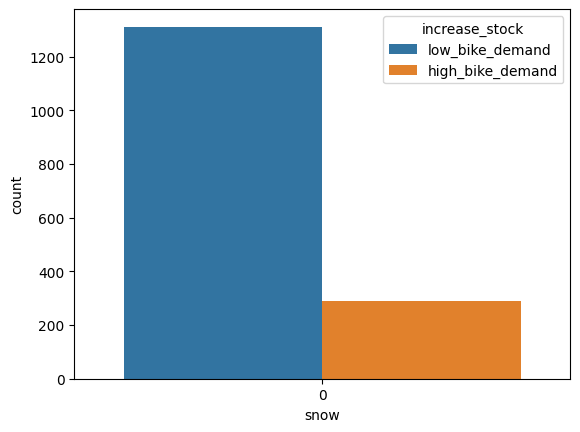
\includegraphics[width=0.5\textwidth]{Code/Plots/snow.png}
   }\hfill
     \subfloat[\label{fig:summertime}Increase stock during summertime.]{
       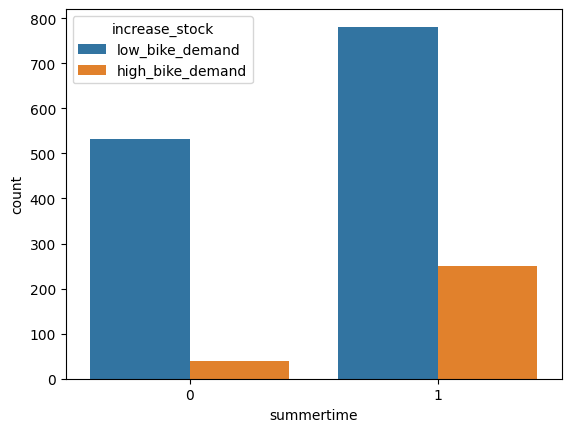
\includegraphics[width=0.5\textwidth]{Code/Plots/summertime.png}
    }      
\end{figure}



\end{enumerate}

\end{enumerate}
\subsection{Treating the Data}

Data set analysis was explored based on the provided inputs. It was possible to conclude that by removing some data from the given input the accuracy of the models can be increased. This happens because certain data does not have as much correlation with the output, so the results may differ. Therefore, the following data was removed from the inputs to obtain better results:

\begin{equation}
RemovedInputs = visibility, snowdepth, precip
\end{equation}

The provided input data was divided into training data, testing data and validation data applied to all implemented models. The training data is 75\%, the test data is 15\% and the validation data is 15\%, of the total amount of the input data (1600 data points). It is important to mentioned that the inputs was re-scaled in order to apply in the methods to do the prediction.


\section{Predictions}
Throughout the project, we experimented with different model families to figure out which one would best suit the problem at hand. This section gives a brief overview of the model families we experimented with and lastly presents which one we decided as the most suitable prediction to the given problem. The follows models was analysed: Logistic Regression, Discriminant analysis (LDA and QDA), K-nearest neighbor, Tree-based methods (classification trees, random forests, bagging) and Boosting (adaptative and gradient).


\subsection{Logistic Regression}

Logistic Regression  modelling conditional class probabilities. It is a model for classification whose decision boundaries are linear. The given prediction has been made for binary classification. An analysis was made in order to choose the appropriate decision threshold "r" to minimises the so-called misclassification rate for the given application. The analysis was made considering the accuracy and the confusion matrix focusing in improve the model. It is possible to see in Figure \ref{fig:thresholds_versus_accuracy} the different accuracy values found when the decision threshold "r" is chosen in the [0,1] interval.

% \begin{figure}[htb!]
% \includegraphics[width=12cm]{...}
% \caption{Analysis of the appropriate decision threshold "r".}
% \label{fig:thresholds_versus_accuracy}
% \end{figure}

The Confusion matrix can be seen in Figure \ref{fig:cmlg}.

\begin{figure}[H]
    \centering
    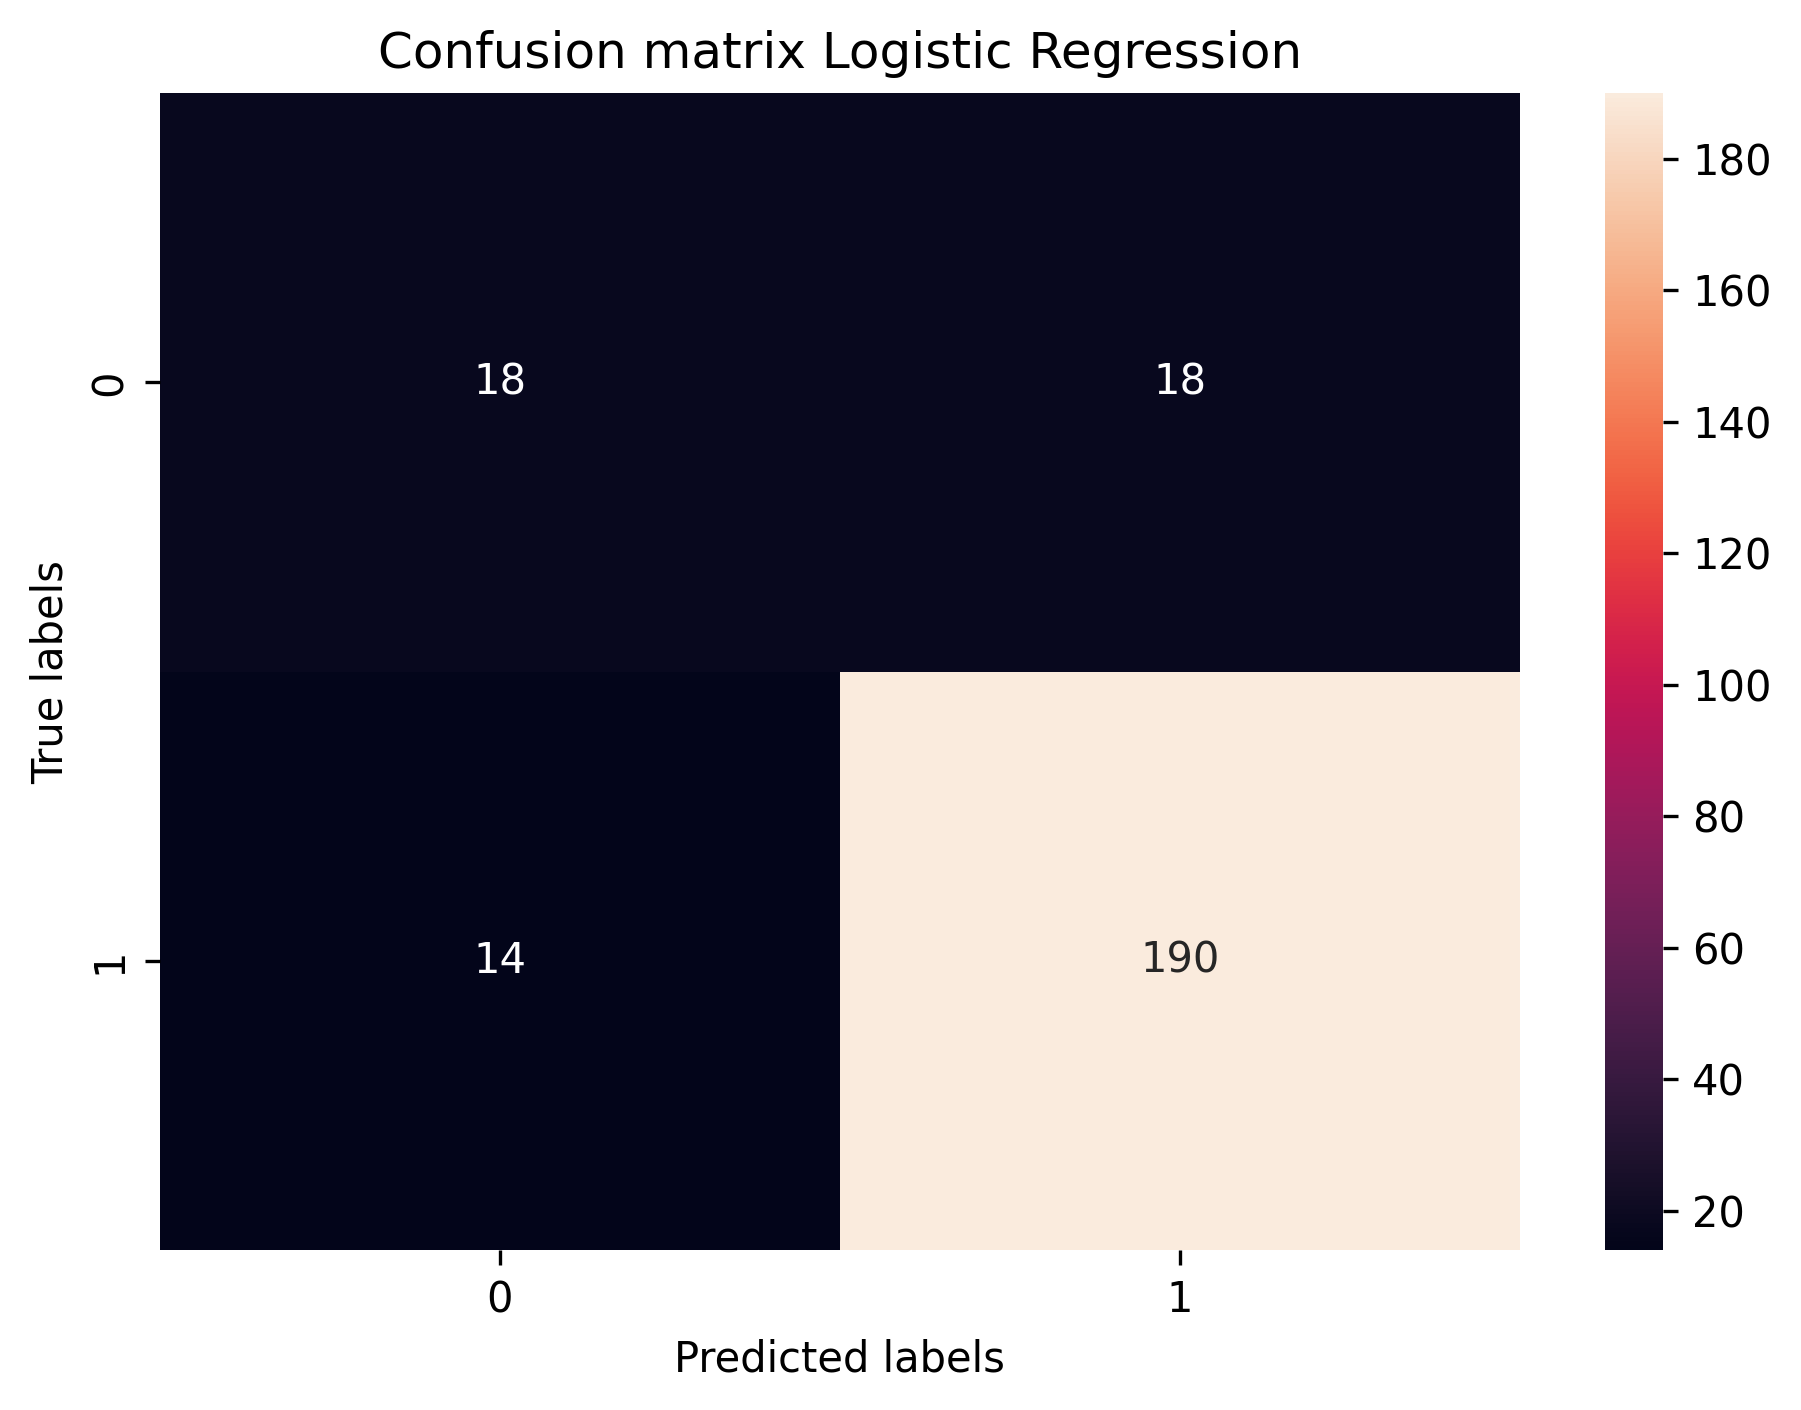
\includegraphics[width=0.5\linewidth]{Report/Images/confusion_matrix_marina_regression.png}
    \caption{Confusion matrix - Logistic Regression}
    \label{fig:cmlg}
\end{figure}


\subsection{Discriminant Analysis (LDA and QDA)}

Linear Discriminant Analysis (LDA) is a linear model for classification. It treats training data as though observations of each class are samples from a multidimensional normal distribution. The decision boundary is exactly at the point where the probabilities of each of the classes are equal. LDA is a special case of Discriminant analysis where the covariance matrices of each of the distributions are assumed to be the same.

%When learning a classifier using LDA, a set of three parameters have to be learned, for each of the classes in the data.
%The parameters to be learned for all classes \(1, 2, ..., \boldsymbol{M}\) are the following

%\begin{equation}
%\theta = \left\{ \boldsymbol{\mu}_m, \boldsymbol{\Sigma}_m, \pi_m \right\}_{m=1}^M
%\end{equation}

%Where \(\boldsymbol{\mu}_m, \boldsymbol{\Sigma}_m, \pi_m\) is the class-dependent mean vector, covariance matrix, and prior probability of class \(\boldsymbol{m}\), respectively.

%The parameters are learned by maximizing the log-likelihood of the training data

%\begin{equation}
%\boldsymbol{\hat{\theta}} = \arg\max_{\theta} \ln p(\{\boldsymbol{x}_i,y_i\}_{i=1}^n | \boldsymbol{\theta}).
%\end{equation}

%where \(\{\boldsymbol{x}_i,y_i\}_{i=1}^n\) is the training data.

%The predictions are then made by selecting the class that is most probable

%\begin{equation}
%\hat{y}_* = \arg\max_m p(y = m | \boldsymbol{x}_*)
%\end{equation}

%Where \(p\) is a multivariate normal distribution based on the previously learned parameters.

%LDA was one of the models we explored when experimenting with different model families for the problem at hand. The code written can be found in the appendix TODO REFER TO APPENDIX.

%a) TODO

%b) TODO

%c) TODO

\subsection{K-nearest neighbor}

The K-nearest neighbor prediction method is an update of the 1-nearest neighbour method.

The Confusion matrix can be seen in Figure \ref{fig:cmkn}.


\begin{figure}[H]
		\centering
		\caption{Confusion matrix - K-nearest neighbor.}		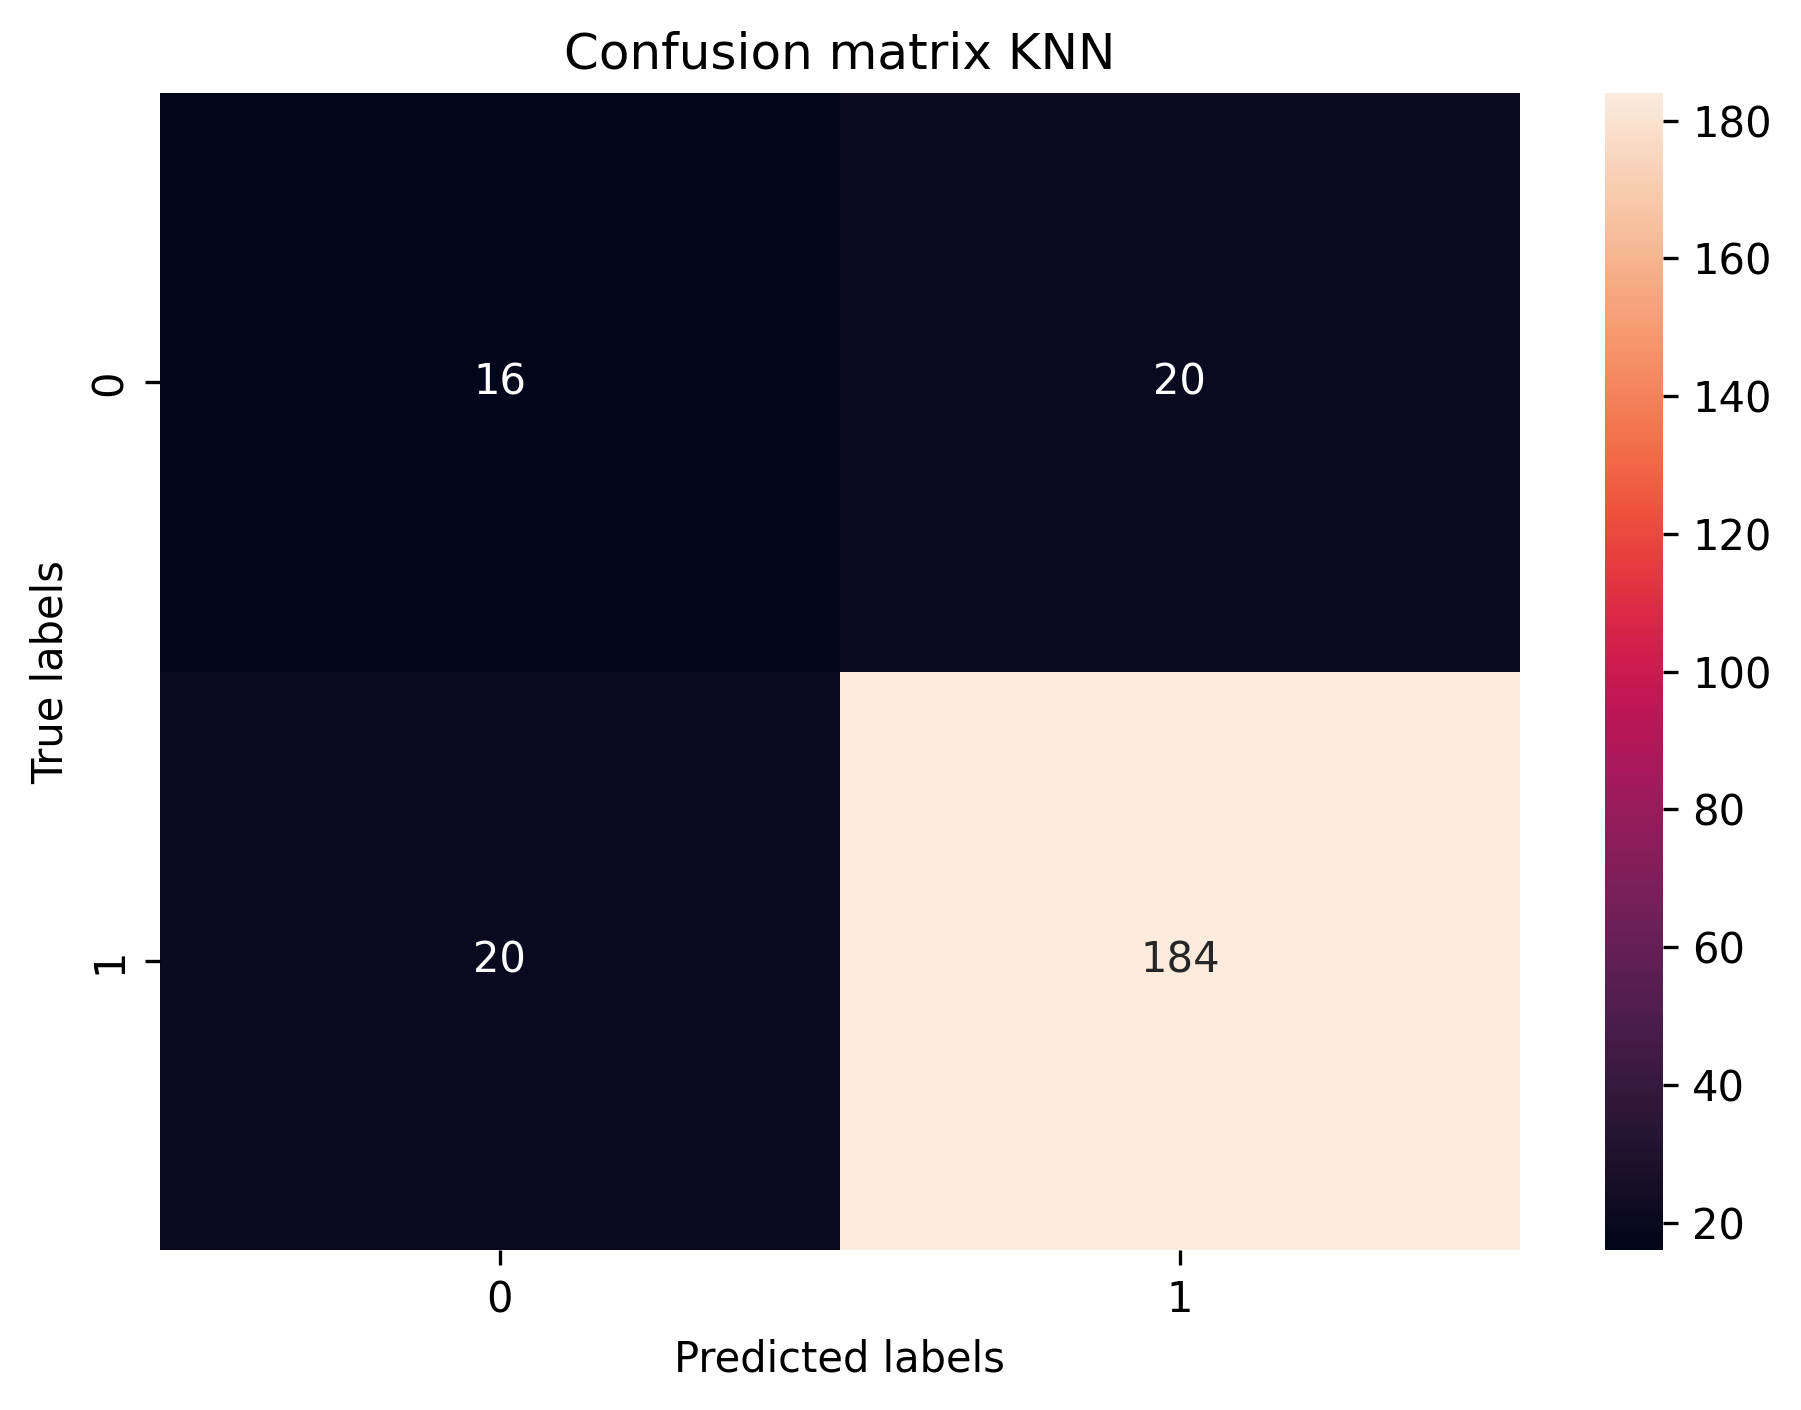
\includegraphics[width=0.5\linewidth]{Report/Images/confusion_matrix_renan_knn.png}
	\label{fig:cmkn}
	\end{figure}

\subsection{Comparison between all implement methods}

%%fazer tabela


\section{Conclusion}

\section*{References}


References follow the acknowledgments. Use unnumbered first-level heading for
the references. Any choice of citation style is acceptable as long as you are
consistent. It is permissible to reduce the font size to \verb+small+ (9 point)
when listing the references.
Note that the Reference section does not count towards the page limit.
\medskip


{
\small


[1] Alexander, J.A.\ \& Mozer, M.C.\ (1995) Template-based algorithms for
connectionist rule extraction. In G.\ Tesauro, D.S.\ Touretzky and T.K.\ Leen
(eds.), {\it Advances in Neural Information Processing Systems 7},
pp.\ 609--616. Cambridge, MA: MIT Press.


[2] Bower, J.M.\ \& Beeman, D.\ (1995) {\it The Book of GENESIS: Exploring
  Realistic Neural Models with the GEneral NEural SImulation System.}  New York:
TELOS/Springer--Verlag.


[3] Hasselmo, M.E., Schnell, E.\ \& Barkai, E.\ (1995) Dynamics of learning and
recall at excitatory recurrent synapses and cholinergic modulation in rat
hippocampal region CA3. {\it Journal of Neuroscience} {\bf 15}(7):5249-5262.
}


%%%%%%%%%%%%%%%%%%%%%%%%%%%%%%%%%%%%%%%%%%%%%%%%%%%%%%%%%%%%


%%%%%%%%%%%%%%%%%%%%%%%%%%%%%%%%%%%%%%%%%%%%%%%%%%%%%%%%%%%%


\appendix


\section{Appendix}


Optionally include extra information (complete proofs, additional experiments and plots) in the appendix.
This section will often be part of the supplemental material.


\end{document}